\documentclass{beamer}

\usetheme[numbering=fraction,block=fill]{metropolis}

\usepackage{mathrsfs}
\usepackage{booktabs}
\usepackage{tikz-cd}

\font\maljapanese=dmjhira at 1.6ex

\newcommand{\twitter}{
\includegraphics[width=10pt]{twitter.png}\,\,\,\texttt{@tjohnhos}}
\renewcommand{\matrix}{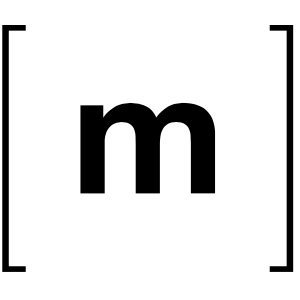
\includegraphics[width=10pt]{matrix.png}\,\,\,\texttt{@thosgood:matrix.org}}

\title{Twisting cochains and twisted complexes}
\subtitle{Simplicial methods in complex-analytic geometry}
\author{Tim Hosgood}
\institute{Université d'Aix-Marseille\\\url{https://thosgood.github.io}\\[1em]\twitter\\\matrix}
\date{24/07/19}

\begin{document}
\begin{frame}
    \titlepage
\end{frame}

\begin{frame}\frametitle{Plan}
    \vspace{1em}
    \tableofcontents
\end{frame}


\section{History}

    \begin{frame}\frametitle{First steps}
        \begin{itemize}
            \item Edgar H Brown. ``Twisted tensor products, I''. In: \emph{Annals of Mathematics} 69.1 (1959), pp.~223--246.
            \item John C Moore. ``Differential homological algebra''. In: \emph{Actes du Congres International des Mathématiciens} 1 (1970), pp.~335--339.
        \end{itemize}
    \end{frame}

    \begin{frame}\frametitle{Coherent sheaves}
        \begin{itemize}
            \item Domingo Toledo and Yue Lin L Tong. ``A parametrix for $\delta$ and Riemann-Roch in Čech theory''. In: \emph{Topology} 15.4 (1976), pp.~273--301.
            \item Domingo Toledo and Yue Lin L Tong. ``Duality and Intersection Theory in Complex Manifolds. I''. In: \emph{Mathematische Annalen} 237 (1978), pp.~41--77.
            \item Nigel R O'Brian, Domingo Toledo, and Yue Lin L Tong. ``The Trace Map and Characteristic Classes for Coherent Sheaves''. In: \emph{American Journal of Mathematics} 103.2 (1981), pp.~225--252.
        \end{itemize}
    \end{frame}

    \begin{frame}\frametitle{Triangulation and stability}
        \begin{itemize}
            \item A I Bondal and M M Kapranov. ``Enhanced Triangulated Categories''. In: \emph{Math. USSR Sbornik} 70.1 (1991), pp.~1--15.
            \item Giovanni Faonte. \emph{Simplicial nerve of an A-infinity category}. 2015. arXiv: 1312.2127v2 [math.AT].
        \end{itemize}
    \end{frame}

    \begin{frame}\frametitle{Nomenclature}
        \begin{lemma}
            Let $x\in\{\text{twisting},\text{twisted}\}$ and $y\in\{\text{cochain},\text{complex}\}$.

            Then there exists somebody who uses ``$x\,y$'' to denote what you call ``$x^c\,y^c$''.
        \end{lemma}

        \begin{corollary}
            Sometimes it can be hard to figure out what people mean.
        \end{corollary}
        
        \pause

        I like ``twisting cochain'' for the topological Čech definition, which is a special case of a ``twisted complex'', defined in the dg-categorical setting.

        \pause

        But that's very possibly just me.
    \end{frame}


\section{Twisting cochains (OTT)}

    \subsection{The bicomplex}

        \begin{frame}\frametitle{Nice spaces}
            \begin{definition}[Stein spaces]
                A complex-analytic\footnote{analytic = $\mathcal{O}_Y$ is holomorphic functions, $Y$ has the $\mathbb{C}^n$-induced topology; algebraic = $\mathcal{O}_Y$ is algebraic functions, $Y$ has the Zariski topology.} manifold $Y$ is said to be \emph{Stein} if it is
                \begin{enumerate}
                    \item \emph{holomorphically convex}; and
                    \item \emph{holomorphically separable}.
                \end{enumerate}
            \end{definition}

            \pause

            \begin{block}{Motto}
                Stein things are nice.
            \end{block}

            \pause

            Throughout, $X$ is a complex-analytic manifold with a nice\footnote<3>{\emph{Locally finite}, \emph{Stein}, and \emph{trivialising} (for the bundles in question).} cover $\mathcal{U}=\{U_\alpha\}_{\alpha\in I}$.
        \end{frame}

        \begin{frame}\frametitle{Endomorphisms of bounded-graded modules}
            Let $V=\{V_\alpha^\bullet\}$ be a collection of \emph{bounded-graded $\mathcal{O}_{U_\alpha}$-modules}:
            \begin{equation*}
                V_\alpha^\bullet = \bigoplus_{q\in\mathbb{N}}V_\alpha^q\quad\text{such that }V_\alpha^q\text{ is zero for all but finitely many }q.
            \end{equation*}

            \pause

            Think of a bounded chain complex of vector bundles, but without the information of a differential.

            \pause

            \begin{definition}[Endomorphisms]
                The collection of \emph{degree-$q$ endomorphisms $\mathrm{End}^q(V)$ of $V$} is, over each $U_{\alpha_0\ldots\alpha_p}$, given by
                \begin{equation*}
                    \mathrm{End}^q(V)|U_{\alpha_0\ldots\alpha_p} = \bigoplus_{i\in\mathbb{Z}}\mathrm{Hom}\big( V_{\alpha_p}^i|U_{\alpha_0\ldots\alpha_p}, V_{\alpha_0}^{i+q}|U_{\alpha_0\ldots\alpha_p} \big).
                \end{equation*}
            \end{definition}
        \end{frame}

        \begin{frame}\frametitle{Source and target}
            \begin{alertblock}{Warning}
                The maps are from the $\alpha_p$ part to the $\alpha_0$ part.
            \end{alertblock}

            \pause

            We discuss this later.
        \end{frame}

        \begin{frame}\frametitle{The deleted Čech complex}
            \begin{definition}[Deleted Čech complex]
                Define the chain complex $(\hat{\mathscr{C}}^\bullet(\mathcal{U},\mathrm{End}^\circ(V)),\hat{\delta})$ by
                \begin{equation*}
                    \hat{\mathscr{C}}^p\big(\mathcal{U},\mathrm{End}^q(V)\big) = \bigoplus_{(\alpha_0,\ldots,\alpha_p)} \mathrm{End}^q(V)|U_{\alpha_0\ldots\alpha_p}
                \end{equation*}
                (where $\mathrm{End}^q(V)|U_{\alpha_0\ldots\alpha_p}=0$ if $U_{\alpha_0\ldots\alpha_p}=\varnothing$) with the \emph{\textbf{deleted} Čech differential}
                \begin{gather*}
                    \hat{\delta} \colon \hat{\mathscr{C}}^p\big(\mathcal{U},\mathrm{End}^q(V)\big) \to \hat{\mathscr{C}}^{p+1}\big(\mathcal{U},\mathrm{End}^q(V)\big)\\
                    (\hat{\delta}c)_{\alpha_0\ldots\alpha_{p+1}} = \sum_{i=1}^p (-1)^i c_{\alpha_0\ldots\widehat{\alpha_i}\ldots\alpha_{p+1}}.
                \end{gather*}
            \end{definition}
        \end{frame}

        \begin{frame}\frametitle{A notational note}
            We use $\hat{\mathscr{C}}$ and $\hat{\delta}$ for the \emph{deleted} Čech objects and $\check{\mathscr{C}}$ and $\check{\delta}$ for the `full' Čech objects.
        \end{frame}

        \begin{frame}\frametitle{Further structure}
            \begin{itemize}
                \item If $V$ has a differential then this gives us a \emph{bicomplex}.
                \pause
                \item There is a natural multiplication structure given by composition:
                    \begin{equation*}
                        (c^{p,q}\cdot \tilde{c}^{\tilde{p},\tilde{q}})_{\alpha_0\ldots\alpha_{p+\tilde{p}}} = (-1)^{q\tilde{p}} c_{\alpha_0\ldots\alpha_p}^{p,q} \tilde{c}_{\alpha_p\ldots\alpha_{p+\tilde{p}}}^{\tilde{p},\tilde{q}}.
                    \end{equation*}
                \pause
                \item We could define the same complex for an arbitrary bounded graded vector bundle, i.e.
                \begin{equation*}
                    \hat{\mathscr{C}}^p(\mathcal{U},V^q) = \bigoplus_{(\alpha_0,\ldots,\alpha_p)} V_{\alpha_0}^q
                \end{equation*}
                but where the deleted Čech differential only omits the \emph{first} index (but includes the $(p+1)$th).
            \end{itemize}
        \end{frame}

        \begin{frame}\frametitle{A brief interlude on bundles}
            A holomorphic vector bundle $E$ on $X$ is described exactly by its \emph{transition maps $g_{\alpha\beta}\in\mathrm{GL}(n,\mathbb{C})$}, which describe the change in trivialisation from over $U_\beta$ to over $U_\alpha$.

            \pause

            These transition maps satisfy two conditions:

            \pause
            
            \begin{enumerate}
                \item $g_{\alpha\beta}g_{\beta\gamma}=g_{\alpha\beta}$ (the \emph{cocycle} condition); and
                \pause
                \item $g_{\alpha\alpha}=\mathrm{id}$ (the \emph{invertibility} condition).
            \end{enumerate}

            \pause

            Note that these are maps from $E|U_{\alpha_p}$ to $E|U_{\alpha_0}$ in the specific case where $p=1$.
        \end{frame}

        \begin{frame}\frametitle{Rewriting the cocycle condition}
            Thinking of $g_{\alpha\beta}$ as an element of $\hat{\mathscr{C}}^1(\mathcal{U},E)$, we see that
            \begin{gather*}
                (\hat{\delta}g)_{\alpha\beta\gamma} = -g_{\alpha\gamma}\\
                (g\cdot g)_{\alpha\beta\gamma} = g_{\alpha\beta}g_{\beta\gamma}.
            \end{gather*}

            \pause

            This means that we can rewrite the cocycle condition as
            \begin{equation*}
                \hat{\delta}g + g\cdot g = 0,
            \end{equation*}
            which looks like the \emph{Maurer-Cartan equation} (an observation to which we will later return).
        \end{frame}

        \begin{frame}\frametitle{Twisting cochains}
            \begin{definition}[Twisting cochains]
                A \emph{(holomorphic) twisting cochain over $V$} is a formal sum
                \begin{equation*}
                    \mathrm{a} = \bigoplus_{k\in\mathbb{N}} \mathrm{a}^{k,1-k}
                \end{equation*}
                where $\mathrm{a}^{k,1-k}\in\hat{\mathscr{C}}^k(\mathcal{U},\mathrm{End}^{1-k}(V))$ such that
                \begin{enumerate}
                    \item $\hat{\delta}\mathrm{a} + \mathrm{a}\cdot\mathrm{a} = 0$; and
                    \item $\mathrm{a}_{\alpha\alpha}^{1,0}=\mathrm{id}$.
                \end{enumerate}
            \end{definition}

            \pause

            The invertibility condition ``should'' really be weakened by asking only that $\mathrm{a}_{\alpha\alpha}^{1,0}$ be \emph{homotopic} to the identity.
        \end{frame}

        \begin{frame}\frametitle{Twisting cochains (cont.)}
            \begin{alertblock}{Warning}
                The multiplication is \textbf{not} simply component-wise: it is given by taking all possible combinations, i.e.
                \begin{equation*}
                    (\mathrm{a}\cdot\mathrm{b})^{p,s} = \bigoplus_{\substack{q+q'=p\\t+t'=s}} \mathrm{a}^{q,t}\cdot\mathrm{b}^{q',t'}.
                \end{equation*}
            \end{alertblock}

            \pause
            
            \begin{itemize}
                \item It might be the case that all but finitely many of the $\mathrm{a}^{k,1-k}$ are zero, but \textbf{never} $\mathrm{a}^{1,0}$, since it has to be the identity on $\alpha\alpha$.
                \pause
                \item If $V$ has a differential then $\mathrm{a}$ is an element of total degree $1$.
                \pause
                \item We haven't said \emph{when} twisting cochains exist, but under pretty mild assumptions they always do (by an inductive construction).
            \end{itemize}
        \end{frame}

        \begin{frame}\frametitle{Unpacking the definition}
            \begin{description}
                \item[($k=0$) $\rightsquigarrow$] $\mathrm{a}_{\alpha}^{0,1}\cdot\mathrm{a}_{\alpha}^{0,1}=0$, which tells us that $\mathrm{a}_{\alpha}^{0,1}$ is a \emph{differential on $V_\alpha^\bullet$}.
                \pause
                \item[($k=1$) $\rightsquigarrow$] $\mathrm{a}_{\alpha}^{0,1}\cdot\mathrm{a}_{\alpha\beta}^{1,0} = \mathrm{a}_{\alpha\beta}^{1,0}\cdot\mathrm{a}_{\beta}^{0,1}$, which tells us that we have a \emph{chain map of chain complexes}
                    \begin{equation*}
                        \mathrm{a}_{\alpha\beta}^{1,0} \colon \big(V_\beta^\bullet|U_{\alpha\beta},\mathrm{a}_\beta^{0,1}\big) \to \big(V_\alpha^\bullet|U_{\alpha\beta},\mathrm{a}_\alpha^{0,1}\big)
                    \end{equation*}
                \vspace{-1.5em}
                \pause
                \item[($k=2$) $\rightsquigarrow$] $-\mathrm{a}_{\alpha\gamma}^{1,0} + \mathrm{a}_{\alpha\beta}^{1,0}\cdot\mathrm{a}_{\beta\gamma}^{1,0} = \mathrm{a}_{\alpha}^{0,1}\cdot\mathrm{a}_{\alpha\beta\gamma}^{2,-1} + \mathrm{a}_{\alpha\beta\gamma}^{2,-1}\cdot\mathrm{a}_{\gamma}^{0,1}$, which says that $\mathrm{a}_{\alpha\beta\gamma}^{2,-1}$ witnesses a \emph{chain homotopy} between $\mathrm{a}_{\alpha\gamma}^{1,0}$ and $\mathrm{a}_{\alpha\beta}^{1,0}\cdot\mathrm{a}_{\beta\gamma}^{1,0}$.
                    On $\alpha\beta\alpha$ and $\beta\alpha\beta$ this tells us that $\mathrm{a}_{\alpha\beta}^{1,0}$ and $\mathrm{a}_{\beta\alpha}^{1,0}$ are \emph{chain homotopic inverses}, i.e. \emph{quasi-isomorphism}.
            \end{description}
        \end{frame}

        \begin{frame}\frametitle{Unpacking the definition (cont.)}
            \begin{description}
                \item[($k\geqslant3$) $\rightsquigarrow$] some sort of `higher homotopic gluings', whatever this might mean.
            \end{description}

            \pause

            This is one of the things that we want to formalise!

            \pause

            \begin{block}{Extra-curricular}
                By taking (internal) homology we obtain something strict: a complex of \emph{coherent sheaves} $\mathrm{H}^\bullet(\mathrm{a})$.
                This is because quasi-isomorphisms become strict isomorphisms in homology.

                We can use this fact to construct twisting cochains that resolve coherent sheaves by taking \emph{local} resolutions by vector bundles.
            \end{block}
        \end{frame}

    \subsection{The total complex}

        \begin{frame}\frametitle{The total differential}
            \begin{lemma}
                For any $\mathrm{a}\in\mathrm{Tot}^1\hat{\mathscr{C}}^\bullet(\mathcal{U},\mathrm{End}^\circ(V))$, the map
                \begin{align*}
                    \mathrm{D}_\mathrm{a} \colon \mathrm{Tot}^r\hat{\mathscr{C}}^\bullet(\mathcal{U},V^\circ) &\to \mathrm{Tot}^{r+1}\hat{\mathscr{C}}^\bullet(\mathcal{U},V^\circ)\\
                    c &\mapsto \hat{\delta}c+c\cdot\mathrm{a}
                \end{align*}
                defines a differential (i.e. squares to zero) if and only if $\mathrm{a}$ is a twisting cochain.
            \end{lemma}
            \begin{proof}
                (Tedious) definition chasing.
            \end{proof}
        \end{frame}

        \begin{frame}\frametitle{The total differential (cont.)}
            We can actually define twisting cochains in a different way using this lemma (but we won't do so today).

            \pause

            But this approach lets us think of a twisting cochain as a \emph{first-order perturbation of the deleted Čech differential}.
        \end{frame}

        \begin{frame}\frametitle{Examples}
            \begin{example}
                Look at the most trivial example: let $V$ be an \emph{ungraded} vector bundle, and $\mathrm{a} = \mathrm{a}^{0,1}+\mathrm{a}^{1,0}$, where $\mathrm{a}_{\alpha}^{0,1} = \mathrm{id}_{V_\alpha}$, and the $\mathrm{a}^{1,0}$ are the transition maps.
                Then
                \begin{equation*}
                    (\mathrm{D}_\mathrm{a}c)_{\alpha_0\ldots\alpha_{p+1}} = \mathrm{a}_{\alpha_0\alpha_1}^{1,0}c_{\alpha_1\ldots\alpha_{p+1}} + \sum_{i=1}^{p+1}(-1)^i c_{\alpha_0\ldots\widehat{\alpha_i}\ldots\alpha_{p+1}}.
                \end{equation*}

                \pause

                We can't use the full Čech differential on $\hat{\mathscr{C}}^\bullet(\mathcal{U},V^\circ)$ because everything has to lie over $U_{\alpha_0}$, but this total differential solves that problem --- $\mathrm{a}_{\alpha_0\alpha_1}^{1,0}$ is a (quasi-)isomorphism.

                \pause

                A spectral-sequence argument shows that, in fact, $\mathrm{D}_\mathrm{a}$ here really is `the same as' the full Čech differential.
            \end{example}
        \end{frame}

        \begin{frame}\frametitle{Examples (cont.)}
            \begin{example}
                Now look at a slightly-less trivial example: let $V^\bullet$ consist of \emph{complexes} $(V_\alpha^\bullet,\mathrm{d}_\alpha)$ of vector bundles, and $\mathrm{a} = \mathrm{a}^{0,1}+\mathrm{a}^{1,0}$, where $\mathrm{a}_{\alpha}^{0,1} = \mathrm{d}_\alpha$, and the $\mathrm{a}^{1,0}$ are the transition maps.
                Then
                \begin{align*}
                    (\mathrm{D}_\mathrm{a}c)_{\alpha_0\ldots\alpha_{p+1}} &= (-1)^p\mathrm{a}_{\alpha_0}^{0,1}c_{\alpha_0\ldots\alpha_p} + \mathrm{a}_{\alpha_0\alpha_1}^{1,0}c_{\alpha_1\ldots\alpha_{p+1}}\\
                    &\qquad+\sum_{i=1}^{p+1}(-1)^i c_{\alpha_0\ldots\widehat{\alpha_i}\ldots\alpha_{p+1}}.
                \end{align*}

                \pause
                
                Identifying the second and third terms with the full Čech differential, as before, gives the usual total differential of the Čech bicomplex:
                \begin{equation*}
                    \mathrm{D}_\mathrm{a} = \check{\delta} \pm \mathrm{d}_V.
                \end{equation*}
            \end{example}
        \end{frame}

        \begin{frame}\frametitle{Why this emphasis on the first index?}
            \begin{itemize}
                \item Transition maps naturally go from $\alpha_p$ to $\alpha_0$.
                \pause
                \item We want to be able to compare local things, and we need to pull everything back to lie over the same open set in order to do so.
            \end{itemize}
        \end{frame}

    \subsection{Maurer-Cartan}

        \begin{frame}\frametitle{The Maurer-Cartan equation in other fields}
            \begin{table}
                \begin{tabular}{p{1.8cm}cp{3.9cm}}\toprule
                    Subject & Equation & Interpretation\\\midrule
                    Differential geometry & $F_\nabla = \mathrm{d}A + A\cdot A$ & curvature of a Koszul connection\footnote{Here be Christoffel symbols.}\\[.5em]
                    Gauge theory & $\Omega = \mathrm{d}A + \frac12[A\wedge A]$ & curvature of a principal connection\\[.5em]
                    Deformation theory & $\partial a+\frac12[a,a]$ & deformations of f.d. associative $k$-algebras with unit\footnote{There is also the beautiful fact (that we won't explain at all) that $\mathrm{MC}(A\otimes\mathfrak{g}) \simeq \mathrm{Hom}_\mathsf{dgAlg}(\mathrm{CE}(\mathfrak{g}),A)$.}
                    \\\bottomrule
                \end{tabular}
            \end{table}
        \end{frame}

        \begin{frame}\frametitle{Flatness}
            \begin{block}{Motto}
                Solutions to (i.e. zeros of) the Maurer-Cartan equation are always (in some sense) \emph{flat objects}.
            \end{block}
        \end{frame}

    \subsection{Strictification}

        \begin{frame}\frametitle{Can we strictify?}
            No.\footnote{But sort of, yes.}
        \end{frame}


\section{Twisted complexes (BK)}
    
    \subsection{Pretriangulated, triangulated, and stable}

        \begin{frame}\frametitle{Stability}
            \begin{block}{Motto}
                \emph{Pretriangulated dg-categories} are those whose homotopy category is \emph{triangulated}, where \emph{triangulated} denotes the structure left over from taking the homotopy category of a \emph{stable $(\infty,1)$-category}.\footnote{Loop spaces and suspensions form an equivalence.}
            \end{block}
        \end{frame}

        \begin{frame}\frametitle{Stability (cont.)}
            \begin{alertblock}{Problem}
                There is no reason for an arbitrary dg-category to be pretriangulated, which means that homotopy theorists might be unhappy.
                This is bad.
            \end{alertblock}

            \pause

            \begin{block}{Solution}
                Twisted complexes à la Bondal and Kapranov.
            \end{block}
        \end{frame}

        \begin{frame}\frametitle{dg-categories}
            \begin{definition}
                A \emph{dg-category} is a category enriched over chain complexes.
                That is, the hom-sets are hom-\emph{complexes}.
            \end{definition}

            \pause

            \begin{definition}
                Let $\mathcal{A}$ be a dg-category.
                Then a \emph{twisted complex $\mathfrak{C}$ over $\mathcal{A}$} is a collection
                \begin{equation*}
                    \mathfrak{C} = \{E_i\in\mathcal{A},q_{ij}\colon E_i\to E_j\mid i,j\in\mathbb{Z}\}
                \end{equation*}
                such that
                \begin{itemize}
                    \item all but finitely many of the $E_i$ are zero;
                    \item the $q_{ij}$ are of degree $i-j+1$; and
                    \item $\mathrm{d}q_{ij}+\sum_{s\in\mathbb{Z}} q_{sj}q_{is}=0$.
                \end{itemize}
            \end{definition}
        \end{frame}

        \begin{frame}\frametitle{The main result}
            \begin{theorem}
                Given a dg-category, the smallest dg-category containing it in which we can define shifts and functorial cones is exactly its category of twisted complexes.

                \pause

                Further, if the original dg-category is pretriangulated then this embedding is a quasi-equivalence (which lets us pull back the shift and the cones, which descend exactly to a triangulated structure on the homotopy category).

                \pause

                We can also use the \emph{simplicial nerve} to construct stable $(\infty,1)$-categories.
            \end{theorem}
        \end{frame}
    
    \subsection{Generalisation of twisting cochains}

        \begin{frame}\frametitle{Twisting cochains as twisted complexes}
            \begin{alertblock}{Warning}
                It is \textbf{not} the case that, by picking the `right' dg-category $\mathcal{A}$, we can recover the definition of holomorphic twisting cochains from that of twisted complexes.

                \pause

                Rather, twisting cochains are a \emph{specific} case of twisted complexes.
            \end{alertblock}
        \end{frame}

        \begin{frame}\frametitle{Constructing a twisted complex from a twisting cochain}
            \begin{itemize}
                \item Let $\mathcal{A}=\mathsf{dgMod}_B$ where $B=\hat{\mathscr{C}}^\bullet(\mathcal{U},\mathcal{O}_X)$ with differential $\hat{\delta}$.
                \pause
                \item Let $E_0=\hat{\mathscr{C}}^\bullet(\mathcal{U},V)$ (with \textbf{trivial} differential) and $E_i=0$ for all $i\neq0$.
                \pause
                \item We need a degree-1 $B$-linear endomorphism $\mathrm{a}=q_{00}$ of $E_0$ such that $\hat{\delta}\mathrm{a}+\mathrm{a}\mathrm{a}=0$, but we can show that the dg-algebra $\mathrm{End}_B(E_0)$ is exactly $\hat{\mathscr{C}}^\bullet(\mathcal{U},\mathrm{End}^\circ(V))$.
                \pause
                \item Decomposing $\mathrm{a}$ into $\mathrm{a}^{k,1-k}$ we can see that the equation that must be satisfied is exactly what we want.
            \end{itemize}

            \pause

            \begin{block}{Motto}
                Twisting cochains are twisted complexes that are \emph{concentrated in degree zero} and \emph{`projective/free'}.
            \end{block}
        \end{frame}


\section{Other fun things}

    \subsection{The A-infinity Yoneda embedding}

        \begin{frame}\frametitle{The reference}
            Bernhard Keller. \emph{Introduction to A-infinity algebras and modules}. 2001. arXiv: 9910179v2 [math.RA].
        \end{frame}

        \begin{frame}\frametitle{Preliminary definitions}
            \begin{definition}
                \begin{itemize}
                    \item An \emph{$A_\infty$-algebra} is `like a loop space' --- it is a $k$-algebra with a graded derivation, but where associativity of multiplication holds only up to homotopy, which hold only up to homotopy, which...;
                    \item $\mathcal{C}_\infty\mathcal{A}$ is the \emph{category of $A_\infty$-modules} over an $A_\infty$-algebra $\mathcal{A}$;
                    \item $\mathcal{D}_\infty\mathcal{A}$ is the \emph{homotopy category of $\mathcal{C}_\infty\mathcal{A}$}; and $\mathrm{tria}\mathcal{A}$ the ($\mathcal{A}_\infty$-version of the) triangulated subcategory of $\mathcal{D}\mathcal{A}$ generated by the free rank-1 $\mathcal{A}$ module.
                \end{itemize}
                \pause
                In the non-$A_\infty$ case, up to isomorphism, the objects of $\mathrm{tria}\mathcal{A}$ are bounded complexes of finitely-generated free $\mathcal{A}$-modules, and the morphisms "are" homotopy classes of morphisms of complexes.
            \end{definition}
        \end{frame}

        \begin{frame}[fragile]\frametitle{Factorisation of the Yoneda functor}
            \begin{theorem}
                Let $\mathcal{A}$ be an $A_\infty$-category (with strict identities).
                Then the Yoneda functor {\maljapanese\char"48} factors through the $A_\infty$-category $\mathrm{tw}\mathcal{A}$ of twisting cochains
                \begin{equation*}
                    \begin{tikzcd}
                        \mathcal{A}
                            \ar[r,"\text{{\maljapanese\char"48}}_1"]
                            \ar[dr,swap,"\text{{\maljapanese\char"48}}"]
                        & \mathrm{tw}\mathcal{A}
                            \ar[d,"\text{{\maljapanese\char"48}}_2"]\\
                        & \mathcal{C}_\infty\mathcal{A}
                    \end{tikzcd}
                \end{equation*}

                \pause
                
                Further, $\text{{\maljapanese\char"48}}_1$ is (strictly) fully faithful, and $\text{{\maljapanese\char"48}}_2$ induces an equivalence
                \begin{equation*}
                    \mathrm{H}^0\mathrm{tw}\mathcal{A} \xrightarrow{\sim} \mathrm{tria}\mathcal{A}.
                \end{equation*}

                \pause

                This lets us formalise what the $A_\infty$-version of $\mathrm{tw}\mathcal{A}$ really is.
            \end{theorem}
        \end{frame}
    
    \subsection{The bar construction}

        \begin{frame}\frametitle{The set-up}
            \begin{itemize}
                \item dg-coalgebra $(C,\mathrm{d}_C)$ with comultiplication $\Delta$;
                \pause
                \item dg-algebra $(A,\mathrm{d}_A)$ with multiplication $\mu$.
            \end{itemize}

            \pause

            Then a \emph{twisting cochain} is a morphism $\tau\colon C\to A[1]$ such that
            \begin{equation*}
                \mathrm{d}_A\circ\tau + \tau\circ\mathrm{d}_C + \mu\circ(\tau\otimes\tau)\circ\Delta = 0.
            \end{equation*}

            \pause

            Note that this \emph{is} Maurer-Cartan, since the last term is the product $\tau\star\tau$ in the \emph{convolution algebra}.
        \end{frame}

        \begin{frame}\frametitle{The cobar-bar adjunction}
            The \emph{bar-cobar adjunction} is $(\Omega\dashv\mathrm{B})$ between  \emph{cocomplete} dg-coalgebras $\mathsf{dgCog}_{\mathrm{cc}}$ and dg-algebras $\mathsf{dgAlg}$.
            
            \pause

            Given $f\in\mathsf{dgCog}_{\mathrm{cc}}(C,\mathrm{B}A)$ we can define $\tau_f=f\circ\rho$, where $\rho\colon\mathrm{B}A\to A[1]$ is the natural projection.
            Then $\tau_f\colon C\to A[1]$.

            \pause

            Maurer-Cartan then reduces to asking that $f$ is a \emph{chain map} (which is true, by definition).

            \pause

            We can do something similar to then turn $\tau_f$ into a chain map (again, by Maurer-Cartan) $f'\colon\Omega C\to A$.
        \end{frame}

        \begin{frame}\frametitle{Koszul duality and twisted tensor products --- full circle}
            Given some twisting cochain $\tau\colon C\to A[1]$ we can define the \emph{twisted tensor products} $-\otimes_\tau A$ and $-\otimes_\tau C$ on the level of (co)derived categories of (co)modules.

            \pause

            These two functors form an equivalence if and only if
            \begin{equation*}
                A\otimes_\tau C\otimes_\tau A\to A
            \end{equation*}
            is a quasi-isomorphism.

            If this is the case then
            \begin{align*}
                \mathrm{H}_\bullet C &= \mathrm{Tor}_\bullet^A(k,k)\\
                \mathrm{H}^\bullet A &= \mathrm{Ext}_C^\bullet(k,k).
            \end{align*}
        \end{frame}

\end{document}
